\chapter{Oscillators}
Three oscillators form the basis of sound generation in Odin 2. You can choose from a wide variety of different modules, which are capable of a wide palette of sounds, even without any further processing. Initially, Odin 2 starts out with an Analog Osc in slot 1 and none in slot 2 \& 3. 
\vspace{5mm}

\audioparameter{Osc Type}{0}{0}{You can change the module being used with the small dropdown button on the top-right of the osc-module:

\vspace{5mm}
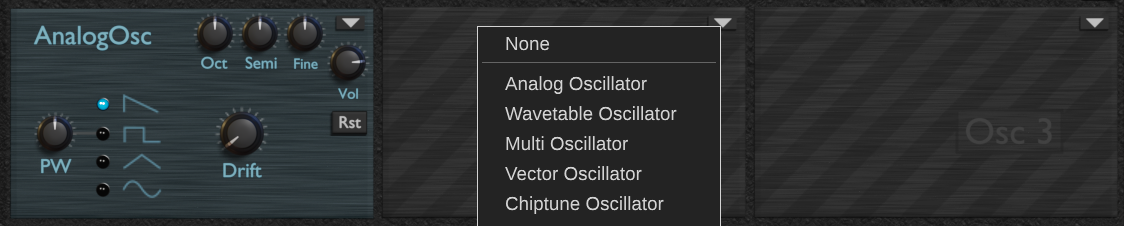
\includegraphics[width=\textwidth]{graphics/osc_selection.png}}

\section{Common Parameters}
There are some controls which are common to all oscillator modules:

\begin{center}
    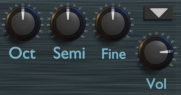
\includegraphics[width=0.3\textwidth]{graphics/osc_common.png}
\end{center}

\audioparameter{Osc Octave}{1}{1}
{Detunes the oscillator in whole octaves.}

\audioparameter{Osc Semitones}{1}{1}
{Detunes the oscillator in semitones.}

\audioparameter{Osc Finetune}{1}{1}
{Detunes the oscillator in cents.}

\audioparameter{Osc Volume}{1}{1}
{Regulates the volume of this oscillator in deciBels. Can be used to shut the oscillator entirely. Modulating this parameter from the \modmatrix  with $-100$ will always shut the sound. Modulating this parameter with $+100$ will raise the sound to 0dB if the current value is smaller than -12dB. If it is bigger than -12dB, it will modulate to +12dB from the current value.}

\begin{center}
    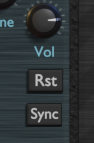
\includegraphics[width=0.1\textwidth]{graphics/osc_common2.png}
\end{center}

\audioparameter{Osc Reset (Rst)}{0}{1}
{Resets the waveform to its initial position each time a key is pressed. This is usefull to get more consistent sounding notes, for example for tight basslines. If this is turned off, the wave will continue where it ended on the last note.}

\audioparameter{Osc Sync}{0}{1}
{This parameter is only available for Osc 2 \& 3. Activating sync will sync this osc to Osc 1. That means each time Osc 1 completes a cycle, this osc is reset to its initial position. The pitch of the oscillator is thereby controlled by Osc 1. This can introduce lots of harmonics, even for soft waveforms like the sinewave.

\vspace{5mm}

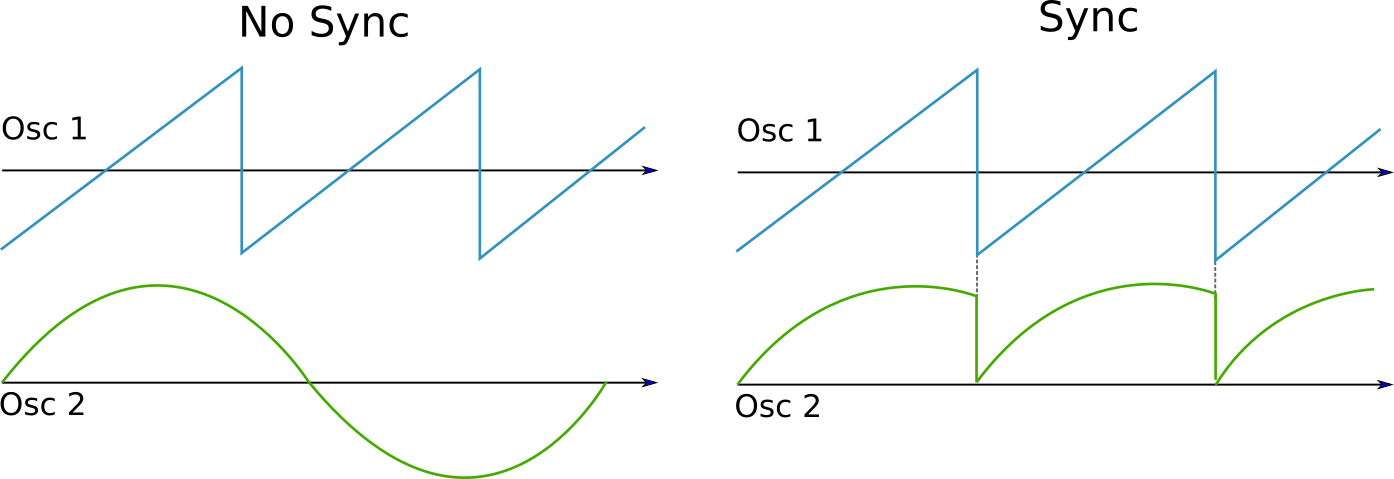
\includegraphics[width=\textwidth]{graphics/osc_sync.png}

Internally, any osc with activated sync will use 3x oversampling to prevent aliasing on the hard resets. Additionally, any osc with enabled sync uses a DC-blocking filter to remove constant offsets in the wave.}

\section{Analog Osc}

\begin{center}
    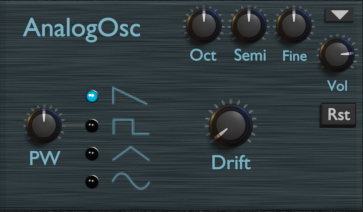
\includegraphics[width=0.5\textwidth]{graphics/analog_osc.png}
\end{center}

The analog osc aims to emulate the sound of classic analog synthesis. The first obvious choice you have is the waveform:

\audioparameter{Analog Waveform}{0}{1}
{

\fat{Sawtooth}:

The classic sawtooth wave. It is very rich in harmonics and forms an excellent starting point for a wide variety of sounds. This particular Sawtooth emulates the way analog syntheizers generate saw-waves. The result is a (phase-corrected) "fat-saw". This variant doesn't rise linearly as the icon would suggest, but in a slight curve, providing a different tonal character.

\fat{Pulse Wave}:

The pulse wave has a thinner sound than the savetooth, sometimes giving the impression of a "hollow" sound body being emulated. The pulse still has a lot of harmonics, making it a common alternative to the sawtooth. The width of the pulse can be adjusted, see the next parameter \fat{Pulse Width}.

\fat{Triangle}:

The triangle wave is much gentler than the saw and pulse waves. It still has a lot of harmonics present though. This wave is well suited for flute like sounds.

\fat{Sine}:

The purest of all waveforms. The sinewave (by its very definition) has no harmonics at all. The resulting sound is very easy on the ears.}

\audioparameter{Pulse Width (PW)}{1}{1}
{This parameter has no effect if the waveform selected is not a pulse. It shifst the duty cycle of the pulse wave, making it stay longer in the lower section for higher values.

\begin{center}
    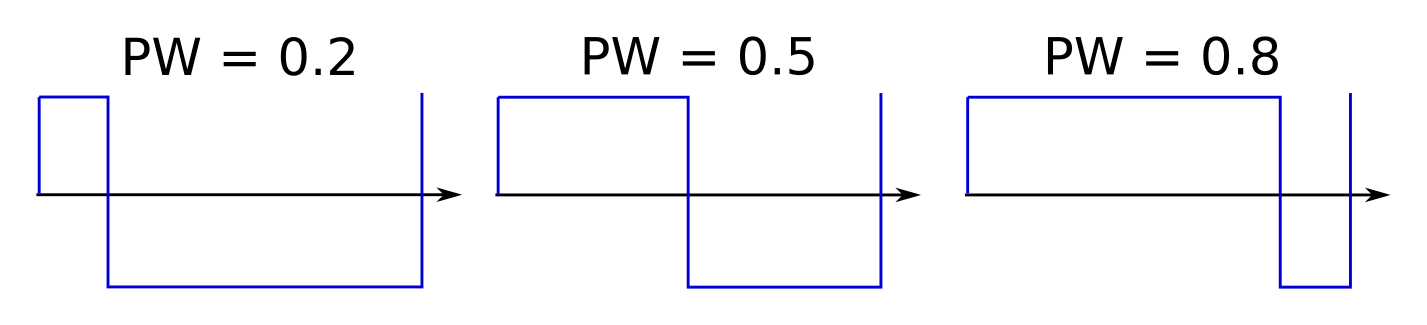
\includegraphics[width=\textwidth]{graphics/PWM.png}
\end{center}

The pulse width control can not be used to shut the sound completely ($PW = 0$ or $PW = 1$), but that can be achieved when modulating via the modmatrix.}

\audioparameter{Drift}{0}{1}
{Analog oscillators tend to not be stable in their frequency. Drift emulates this behaviour by randomly shifting the pitch up and down just a little bit over time. For a single osc, the effect is not very apparent, but becomes clear once two oscillators are used.}

\section{Wavetable Osc}
\begin{center}
    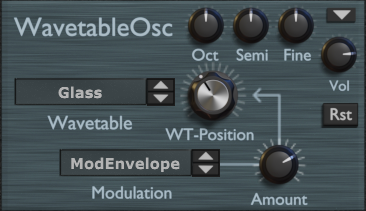
\includegraphics[width=0.5\textwidth]{graphics/wavetable_osc.png}
\end{center}
The Wavetable Osc allows you to create evolving sounds, which feature more than one waveform. Each of the $35$ selectable wavetables consists of four waves itself. You can sweep through these easily by hand or with pre-setup modulation.

\audioparameter{Wavetable}{0}{0}
{Selects which wavetable to be used. A wide variety of sounds is available, starting with analog waveforms, human voice like sounds, additive waves, waveforms taken from instruments and many, many more.}

\audioparameter{Wavetable Position}{1}{1}
{Fades through the four waves in the selected wavetable. A value of $0$ will give the first wave, $0.333$ the second, $0.666$ the third and $1$ the last wave.}

\audioparameter{Modulation}{0}{0}
{Selects a modulation source, which can be used to modulate the Wavetable Position. Modulation Envelope and LFO1 are selectable. Please note that arbitrary modulation sources can be sected when working with the \modmatrix. This slot is merely for a fast and convenient way to set up modulation.}

\audioparameter{Amount}{0}{1}
{Sets the amount of modulation being used to modify the Wavetable Position. Positive and negative values are possible.}

\section{Multi Osc}
\begin{center}
    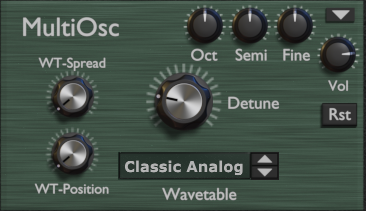
\includegraphics[width=0.5\textwidth]{graphics/multi_osc.png}
\end{center}
The Multi Osc is four oscillators disguised as one. These can be arbitraritly detuned and can even use different waveforms, which results in a thicc, rich sound.

\audioparameter{Detune}{1}{1}
{Detunes the four sub-oscillators agains each other. The detune values are calculated to avoid beating (random phase-cancellation).}

\audioparameter{Wavetable}{0}{0}
{The same as in Wavetable Osc: Selects which wavetable to be used. A wide variety of sounds is available, starting with analog waveforms, human voice like sounds, additive waves, waveforms taken from instruments and many, many more.}

\audioparameter{Wavetable Position}{1}{1}
{The same as in Wavetable Osc: Fades through the four waves in the selected wavetable. A value of $0$ will give the first wave, $0.333$ the second, $0.666$ the third and $1$ the last wave.}

\audioparameter{Wavetable Spread}{1}{1}
{Spreads the four sub-oscillators over the wavetable: The first sub-osc wavetable position will be shifted to the left, the last will be shifted to the right. These shifts happen around the value chosen by Wavetable Position.}

\section{Vector Osc}
\begin{center}
    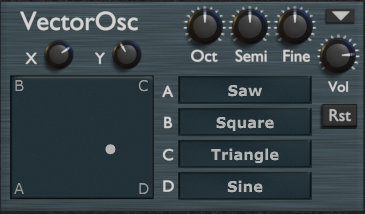
\includegraphics[width=0.5\textwidth]{graphics/vector_osc.png}
\end{center}
The Vector Osc gives even more options for evolving sounds than the Wavetable Osc. Four freely definable waves can be interpolated in a very intuitive graphic way via an XY-pad.

\audioparameter{A, B, C \& D}{0}{0}
{Select the waves to be used. Each of the four letters mark one cornder of the XY-pad, as the graphic suggests. Virtually any waveform from the entire synthesizer can be chosen for any of the corners. This also includes any of the (see \hyperref[wavedraw]{Draw Oscillators}).

When selecting  Draw Osc 1, 2 \& 3, the waves you have drawn in osc slots 1, 2 and \& 3 respectively are used.}

\audioparameter{X \& Y}{1}{1}
{Moves the handle over the XY pad. Each of the corners represent the waveform chosen from the A, B, C and D dropdowns. Moving closer to a corner will make the sound closely relate the waveform of that corner. When being in the corner, the resulting waveform is purely the one selected for that corner. Uses bilinear interpolation to fade through the four tables.}

\section{Chiptune Osc}
\begin{center}
    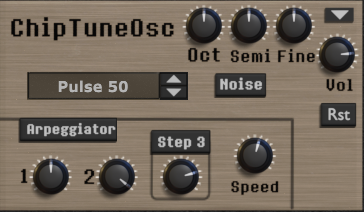
\includegraphics[width=0.5\textwidth]{graphics/chiptune_osc.png}
\end{center}
The Chiptune Osc is an easy way to get nostalgic for your childhood. It aims to emulate the sound of yesteryear while emulating the processing capabilities of a 4-Bit soundchip, like it was used in the Nintendo Entertainment System NES or original Nintendo Gameboy. It also features a simple arpeggiator, with two or three steps being selectable. Whilest being able to produce harmonic sounds, it also features a dedicated chiptune noise module.

\audioparameter{Waveform}{0}{0}
{Lets you select from a variety of waveforms, like you would typically find on the soundchips of yesteryear. Available are a bunch of pulse waves, a triangle, saw and sine variant. All of these waves are limited to a 4Bit resolution (16 steps) on the $Y$-axis. On top of these, you can select any of the \hyperref[chipdraw]{ChipDraw} waves.

To clarify: ChipDraw 1, 2 \& 3 refer to the waves you have drawn in osc slots 1, 2 and \& 3 respectively. You need to apply changes in the ChipdDraw Oscs for the change to take effekt (see \hyperref[chipdraw]{ChipDraw Osc}).}

\audioparameter{Arpeggiator}{0}{1}
{Turns on an internal arpeggiator module, which makes the oscillator jump over predefined semitone values. See the next parameters for specifics.}

\audioparameter{Arp 1, 2 \& 3}{0}{1}
{Select the semitones to be played by the arpeggiator module. For the third step to be used, the next parameter Step 3 needs to be active.}

\audioparameter{Step 3}{0}{1}
{Enables the third step in the arpeggiator. When Step 3 is not active, the arpeggiator will only loop between the first two steps.}

\audioparameter{Speed}{1}{1}
{Sets the speed of the arpeggiator in Hz.}

\audioparameter{Noise}{0}{1}
{Enabling Noise will change stop the output of the selected wavform. Instead, the oscillator will generate a random value to be output each time a cycle is complete. This creates a classic noise effect like it was used on early game consoles. Internally, 3x oversampling is used to remove aliasing on the jumps between values. Note that this noise is dependent on the note being played and has a perceived pitch. It is also possible to use the noise module while the Chiptune arpeggiator is enabled.}

\section{FM Osc}
\begin{center}
    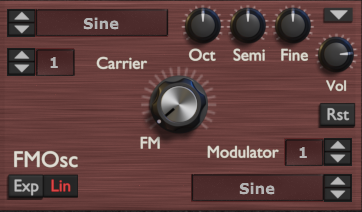
\includegraphics[width=0.5\textwidth]{graphics/fm_osc.png}
\end{center}
The FM Osc is a convenient way to set up Frequency Modulation, or FM. The basic idea behind FM is that you have two oscillators: The carrier and the modulator. The modulator is solely used as a modulation source for the frequency of the carrier. The carrier is the oscillator you will actually hear. While you can set up FM via the \modmatrix as well, the FM osc is the easy way to do it. The theory behind FM is very well documented in other literature, for example on \hyperlink{https://de.wikipedia.org/wiki/FM-Synthese}{Wikipedia}.

FM will usually produce a metallic, bell-like sound.

\audioparameter{Waveform}{0}{0}
{Both carrier and modulator can be assigned a waveform. This will be the actual waveform that the sub-osc is using. Virtually any waveform from the entire synthesizer can be chosen. This also includes any of the (see \hyperref[wavedraw]{Draw Oscillators}).

When selecting  Draw Osc 1, 2 \& 3, the waves you have drawn in osc slots 1, 2 and \& 3 respectively are used.}

\audioparameter{Ratio}{1}{0}
{The numbers above/below the waveform describe the base-frequency relation modulator and carrier have to one another. The frequency of the modulator will alwlays be

\begin{equation}
    f_{mod} = f_{car} \frac{Ratio_{mod}}{Ratio_{car}}
\end{equation}

So for example using the values $Ratio_{mod} = 2$ and $Ratio_{mod} = 1$ will put the modulator one octave (double the frequency) above the carrier. The base freq of the carrier is the pitch played for the note.

Using fractions which are not reducable to "simple" fractions, like $\frac{11}{7}$ will yield wilder results than "simple" ones like $\frac{1}{2}$.

Note that modulating these values from the \modmatrix, allows for fractions which are non-rational (continuous modulation).}

\audioparameter{FM}{1}{1}
{This is where the magic happens: The FM amount controls how deep the modulator modulates the frequency of the carrier. A value of zero will show no modulation at all, so the carrier is playing like a normal osc. When increasing the amount, the sound gets more and more metallic. The range of this parameter can be extended over its natural range via the modmatrix.}

\section{PM Osc}
\begin{center}
    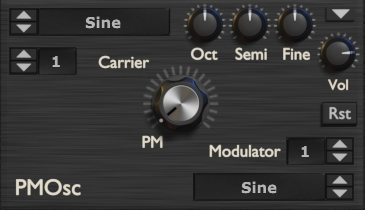
\includegraphics[width=0.5\textwidth]{graphics/pm_osc.png}
\end{center}
PM or Phase Modulation, is closely related to FM or Frequency Modulation. Like the FM Osc, it features a modulator and a carrier oscillator, but this time the modulator modulates the phase of the carrier. When only using sine-waves, the frequency contents generated by FM and PM are indistinguishable.

\audioparameter{Waveform}{0}{0}
{Both carrier and modulator can be assigned a waveform. This will be the actual waveform that the sub-osc is using. Virtually any waveform from the entire synthesizer can be chosen. This also includes any of the (see \hyperref[wavedraw]{Draw Oscillators}).

When selecting  Draw Osc 1, 2 \& 3, the waves you have drawn in osc slots 1, 2 and \& 3 respectively are used.}

\audioparameter{Ratio}{1}{0}
{The numbers above/below the waveform describe the base-frequency relation modulator and carrier have to one another. The frequency of the modulator will alwlays be

\begin{equation}
    f_{mod} = f_{car} \frac{Ratio_{mod}}{Ratio_{car}}
\end{equation}

So for example using the values $Ratio_{mod} = 2$ and $Ratio_{mod} = 1$ will put the modulator one octave (double the frequency) above the carrier. The base freq of the carrier is the pitch played for the note.

Using fractions which are not reducable to "simple" fractions, like $\frac{11}{7}$ will yield wilder results than "simple" ones like $\frac{1}{2}$.

Note that modulating these values from the \modmatrix, allows for fractions which are non-rational (continuous modulation).}

\audioparameter{PM}{1}{1}
{The PM amount controls how deep the modulator modulates the phase of the carrier. A value of zero will show no modulation at all, so the carrier is playing like a normal osc. The range of this parameter can be extended over its natural range via the modmatrix.}

\section{Noise Osc}
\begin{center}
    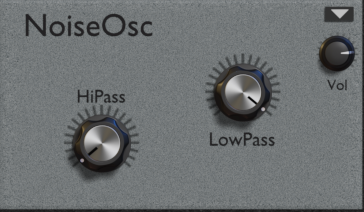
\includegraphics[width=0.5\textwidth]{graphics/noise_osc.png}
\end{center}

The Noise Osc provides a source of noise in Odin 2. The initial noise generation produces white noise. The noise can be further preprocessed by the included lowpass and highpass filters.

\audioparameter{Highpass}{1}{1}
{Sets the cutoff frequency for the included highpass filter. The filter is a first order (6dB / Oct) virtual analog highpass filter.}

\audioparameter{Lowpass}{1}{1}
{Sets the cutoff frequency for the included lowpass filter. The filter is a first order (6dB / Oct) virtual analog lowpass filter.}

\section{WaveDraw Osc}
\label{wavedraw}
\begin{center}
    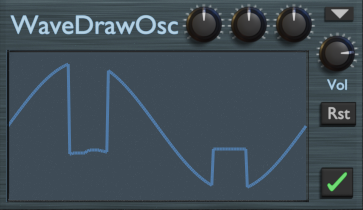
\includegraphics[width=0.5\textwidth]{graphics/wavedraw_osc.png}
\end{center}
The wavedraw osc lets you experiment with waveforms by letting you draw them yourself.

\begin{tcolorbox}[colback=yellow!10!white,
        colframe=white!20!black,
        center,
        valign=top,
        halign=left,
        center title,
        width=\textwidth]

    The changes you make to the waveform will have no effect until you press the apply button on the bottom-right of the oscillator. If this button is red, then there are still unapplied changes to the waveform.
\end{tcolorbox}

The drawn waveform is sampled using 200 discrete steps. When you press the apply button, the waveform is processed into the spectral domain to create a usable wavetable.

\section{ChipDraw Osc}
\label{chipdraw}
\begin{center}
    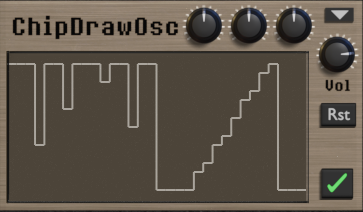
\includegraphics[width=0.5\textwidth]{graphics/chipdraw_osc.png}
\end{center}
The ChipDraw Osc lets you draw a custom chipdraw waveform. It resembles the capabilities of the "custom waveform" on an Nintendo Entertainment System, NES soundsystem. The waveform consists of 32 steps in horizontal direction, which can be offset to 16 values (4Bit) in vertical direction.

\begin{tcolorbox}[colback=yellow!10!white,
        colframe=white!20!black,
        center,
        valign=top,
        halign=left,
        center title,
        width=\textwidth]

    The changes you make to the waveform will have no effect until you press the apply button on the bottom-right of the oscillator. If this button is red, then there are still unapplied changes to the waveform.
\end{tcolorbox}

When you press the apply button, the waveform is processed into the spectral domain to create a usable wavetable.

\section{SpecDraw Osc}
\begin{center}
    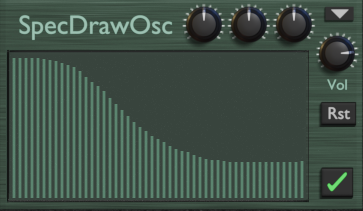
\includegraphics[width=0.5\textwidth]{graphics/specdraw_osc.png}
\end{center}
The SpecDraw Osc opens the sonic capabilities with some \fat{additive synthesis}. Unlike subtractive synthesis, where you filter frequencies from harmonically rich waves, additive synthesis lets you build a sound by stacking up individual harmonics. The n-th harmonic is a sinewave which has n-times the frequency of the base note. The Specdraw Osc lets you draw the amplitude of these sinewaves. The left-most bar represents the fundamental. In the initial state, only this bar ist present, resulting in an overall sinewave osc. As you bring more overtones, the sound gets richer. Addiitve synthesis is capable of creating timbres which are not possible with subtractive synthesis.

\begin{tcolorbox}[colback=yellow!10!white,
        colframe=white!20!black,
        center,
        valign=top,
        halign=left,
        center title,
        width=\textwidth]

    The changes you make to the waveform will have no effect until you press the apply button on the bottom-right of the oscillator. If this button is red, then there are still unapplied changes to the waveform.
\end{tcolorbox}